\documentclass{beamer}

\usepackage[spanish]{babel}
\usepackage{graphicx}
\usepackage{listings}
\usepackage{amsmath}
\usepackage{xcolor}

\lstdefinestyle{myCsharp}{language = [Sharp]C , backgroundcolor = \color{gray!10} , keywordstyle = \color{blue} , commentstyle = \color{green!40!}, stringstyle = \color{orange} , basicstyle = \footnotesize\ttfamily, breaklines = true , tabsize = 4 , columns = fullflexible , showstringspaces = false , escapeinside = {{*@}{@*}}} 

\usetheme{Berlin}
\usecolortheme{whale}
\useoutertheme{shadow}

\AtBeginSection{
    \begin{frame}
        \frametitle{Índice}
        \tableofcontents[currentsection]
    \end{frame}
}

\AtBeginSubsection{
    \begin{frame}
        \begin{frame}
            \frametitle{Índice}
            \tableofcontents[currentsection,currentsubsection]
        \end{frame}
    \end{frame}
}

\title{Presentación Proyecto Moogle}
\author{Kevin Márquez Vega}
\institute{Universidad de La Habana}
\date{\today}

\begin{document}

\lstset{style = myCSharp}

\frame{\titlepage}

\begin{frame}
    \frametitle{Índice}
    \tableofcontents
\end{frame}

\section{Estructura General}

\begin{frame}
    \frametitle{Qué es Moogle?}
    \textit{Moogle} es un motor de búsqueda basado en \textit{tf-idf}, el cual recibe una consulta por parte del usuario 
    y devuelve los resultados más relevantes entre los documentos de su base de datos.
\end{frame}

\begin{frame}
    \frametitle{Cómo se implementa?}
    Está basado en un modelo vectorial, donde se transforman los documentos y la consulta del usuario a vectores, utilizando
    como medida el tf-idf. Luego, a partir de la fórmula de similitud del coseno, se halla el valor del score que representa
    que tan parecido es el documento a la consulta.
\end{frame}


\begin{frame}
    \frametitle{Estructura del algoritmo de Moogle}
    \begin{figure}
        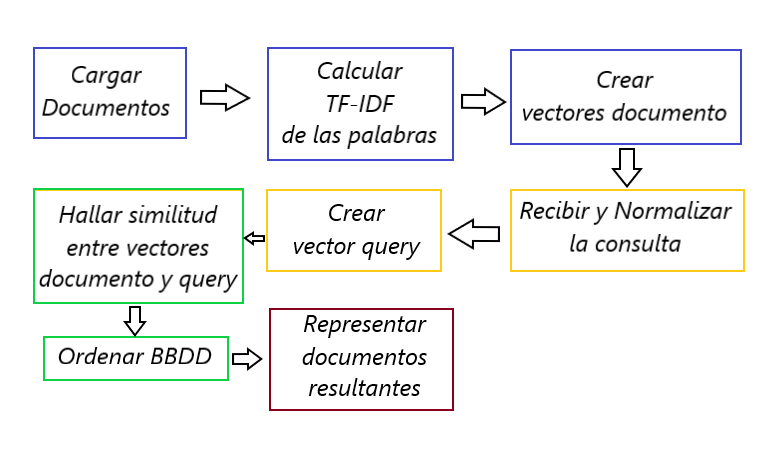
\includegraphics[width = 10cm]{./../images/struct.png}
    \end{figure}
\end{frame}

\section{Creando Vectores Documentos}

\begin{frame}
    \frametitle{Cargar Documentos}

    La función \textit{Search Files} es la encargada de obtener las rutas de los documentos de la base de datos, para poder acceder
    a ellos más tarde. Utiliza múltiples métodos de la clase \textit{Directory} y por cada ruta que encuentra crea un objeto tipo Documento.        
\end{frame}

\begin{frame}[fragile]
    \frametitle{Cargar Documentos}
    \begin{lstlisting} 
public void SearchFiles(string dir)
{            
    dir = Path.Combine(Directory.GetCurrentDirectory() , ".." , dir);
    
    IEnumerable<string> routes = Directory.EnumerateFiles(dir , "*txt" , SearchOption.AllDirectories);
                
    this.docs = new Document[routes.Count()] ;
                
    for( int i = 0 ; i < docs.Length ; i++)
    {
        // por cada ruta se crea un documento
        docs[i] = new Document(routes.ElementAt(i));
    }
}    
    \end{lstlisting}         

\end{frame}

\begin{frame}
    \frametitle{Información necesaria}
    Se necesita saber cuantas veces aparece cada palabra en cada documento. La estructura de datos más útil para ello será
    un diccionario que asocie cada palabra con otra estructura que represente cuantas veces se encuentra en cada documento.
\end{frame}

\begin{frame}
    \frametitle{La mejor solución?}
    Mi primera idea fue utilizar un array pero no sería adecuado debido a la gran cantidad de memoria que ocuparía(sería necesario un
    array por cada palabra con dimensión igual a la cantidad de documentos) y estarían almacenando muchos ceros(los cuales no son relevantes).

    Por eso decidí sustituir los arrays por diccionarios, donde se relaciona el índice del documento con las repeticiones De
    la palabra.
\end{frame}

\begin{frame}
    \frametitle{La mejor solución?}
    
    \begin{figure}
        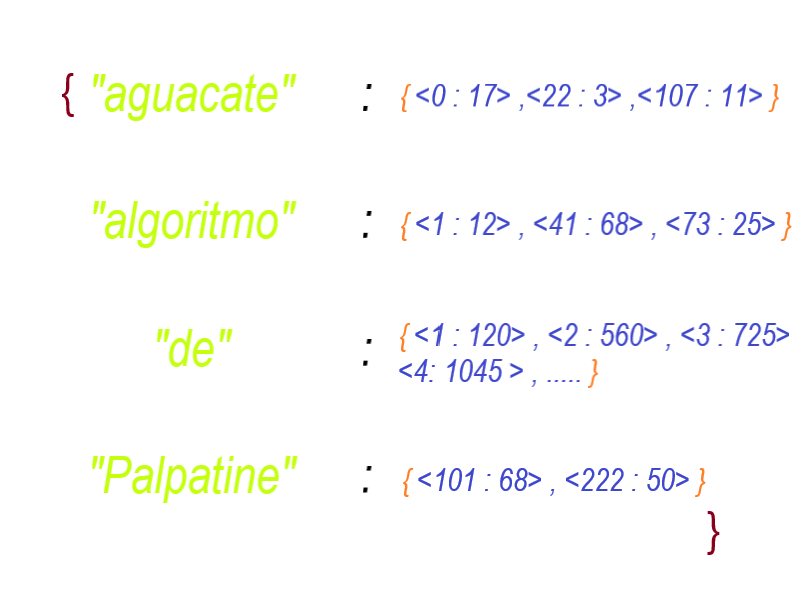
\includegraphics[width = 6cm]{./../images/content.png}
        \caption{Frecuencia de las palabras en los documentos}
    
    \end{figure}
\end{frame}
    
\begin{frame}
    \frametitle{Vectores Documento}
    Siguiendo la misma idea para representar los vectores documento, podemos utilizar un diccionario donde a cada palabra
    se le asocia su relevancia en el documento

    Dicha relevancia estará dada por una medida conocida como \textit{Tf-Idf}(Term Frequency - Inverse Document Frequency).
\end{frame}

\begin{frame}
    \begin{figure}
        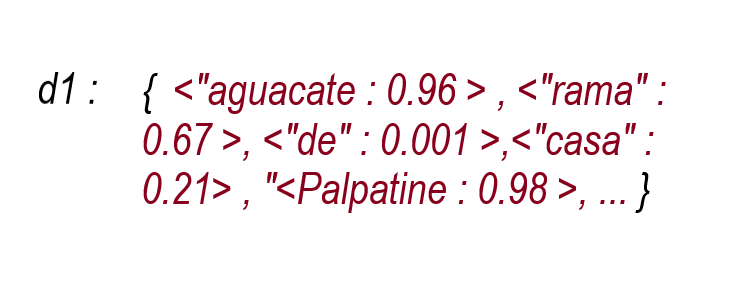
\includegraphics[width = 10cm]{./../images/tfidf.png}
        \caption{Vectores Documento}
    \end{figure}
        
\end{frame}

\begin{frame}
    \frametitle{Calculando el \textit{Tf-Idf}}
    Las fórmulas para calcular dicha medida son : 

    \begin{align*}
        \text{tf-idf} &= \text{tf} \times \text{idf} \\
        \text{tf} = \frac{n}{max_{fq}} &\quad \text{idf} = \log\frac{D + 1}{d_j + 1}
    \end{align*}

    \begin{itemize}
        \item $n$ : repeticiones de la palabra en el documento
        \item $max_{fq}$ : frecuencia maxima en el documento
        \item $D$ : total de documentos
        \item $d_j$ : documentos donde aparece la palabra
    \end{itemize}
    

\end{frame}

\begin{frame}
    \frametitle{Calculando el \textit{Tf-Idf}}
    La manera escogida para almacenar la información facilita el cálculo del \textit{Tf-Idf}
    \begin{figure}
        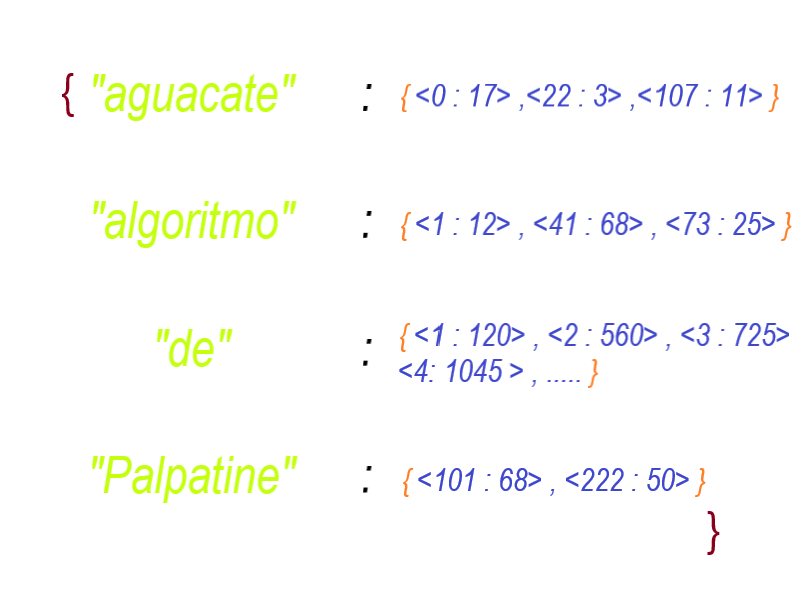
\includegraphics[width = 6cm]{./../images/content.png}
        \caption{Frecuencia de las palabras en los documentos}
    
    \end{figure}
\end{frame}

\section{Trabajando con la Consulta}

\begin{frame}
    \frametitle{Normalizando la consulta}

    Una vez creados los vectores documentos llega el turno de trabajar con la consulta(todo el proceso anterior se 
    realiza antes de que esta sea ingresada).

    Al recibir la consulta, crearemos objetos tipo \textit{Term}, los cuales cuentan con las propiedades : \textit{text} y
    \textit{mod}, las que guardan la palabra y los modificadores que posea respectivamente.
\end{frame}

\begin{frame}
    \frametitle{Normalizando la consulta}
    Al recibir la query, esta debe pasar por un proceso de normalización(para evitar que diferencias en el formato de la palabra
    hagan que el programa interprete la misma como diferentes). \\[20pt]
    
    Por ejemplo : Algoritmo sería tomada diferente a algoritmo.\\[20pt]

    Normalizar la consulta consiste en convertir todas las letras a minúsculas, eliminar simbolos extraños y espacios múltiples
    
\end{frame}

\begin{frame}
    \frametitle{Creando vectores query}
    Repitiendo el proceso realizado con los documentos podemos obtener el vector consulta, el cual será una propiedad de la clase
    Base de Datos.

\end{frame}
\section{Similitud entre vectores}

\begin{frame}
    \frametitle{Comparando vectores}
    Solo faltaría comparar los vectores documento con el vector consulta, lo cual se realizará con la fórmula de similitud
    del coseno, devolviendo el score de cada documento que mientras más cercano a 1 se encuentre, más relevante será el documento
    para la búsqueda(ya que el ángulo entre los vectores se acercará a 0).    
\end{frame}

\begin{frame}
    \frametitle{Similitud del coseno}
    La fórmula de similitud del coseno es la siguiente :
    
    \begin{center}
        $\textit{SimCos(A,B)} = \frac{\sum_{i = 1}^{n}A_iB_i}{\sqrt{\sum_{i = 1}^{n}{A_i}^2} \times \sqrt{\sum_{i = 1}^{n}{B_i}^2}   } $
    \end{center}

    El denominador es conocido como producto escalar, el cual es la sumatoria de los términos con el mismo subíndice en 
    ambos vectores \\[8pt]

    En el programa los subíndices son palabras por tanto bastará con sumar la multiplicación de los pesos de las palabra que se encuentren 
    en ambos vectores.
\end{frame}

\begin{frame}[fragile]
    \frametitle{Producto Escalar}

    \begin{lstlisting} 
public static double EscalarProduct(Vector Q , Vector D)
{
    double suma = 0.0 ;
    foreach(string word in Q.v.Keys)
    {
        if(D.v.ContainsKey(word))
            suma += Q[word] * D[word];
    }
    return suma ;
}
    \end{lstlisting}   
\end{frame}

\begin{frame}[fragile]
    \frametitle{Calculando la norma}
    Para calcular la norma se ha implementado la siguiente función :

    \begin{lstlisting} 
    public double GetNorma()
    {
        double suma = 0.0 ;
        foreach(double weigth in this.v.Values)
        {
            suma += Math.Pow(weigth,2);            
        }
        return Math.Sqrt(suma);
    }
    \end{lstlisting}
\end{frame}

\begin{frame}
    \frametitle{Dando Salida}
    Una vez calculado el score solo faltaría ordenar la base de datos, en este caso a través de un Selection Sort.

    El programa devuelve los mejores 5 documentos(mientras su score sea mayor que 0). Los documentos contienen una función
    llamada \textit{GetSnippet}, la cual localiza la palabra de la consulta más relevante en el documento, y devuelve un pedazo
    de este(un substring de 50 palabras) donde aparece esta.

\end{frame}
\section{Operadores y Sugerencia}
\begin{frame}
    \frametitle{Operadores y Sugerencia}
    Al proyecto se le ha añadido un grupo de funcionalidades extra para hacerlo más completo, como son
    los operadores de importancia, necesidad y prohibición, asi como una sugerencia, la cual ofrece al usuario
    palabras semejantes a las de su búsqueda en caso de que no se encuentren o arrojen pocos resultados.
\end{frame}

\begin{frame}
    \frametitle{Operador de importancia}
    El operador de importancia(*) como su propio nombre indica, aumenta la relevancia de la palabra a la que modifica. Pueden 
    aplicarse varios operadores de importancia sobre la misma palabra aumentando su valor.

    Para su ejecución basta con agregar una variable durante el cálculo del \textit{Tf-Idf} de la consulta : \textit{\textbf{imp}}.

    La cual tendrá como valor por defecto 1 y aumentará según la cantidad de operadores *
\end{frame}

\begin{frame}
    \frametitle{Operadores de necesidad y prohibición}
    Estos operadores realizan operaciones contrarias, pero modifican la búsqueda de manera similar.

    El operador de necesidad(\texttt{\^{}}) obliga a los documentos devueltos a tener la palabra modificada, mientras que 
    el de prohibición(!) los obliga a no tenerla.

    Al calcular la similitud de coseno entre vectores basta con chequear si se cumplen las condiciones de los operadores en 
    el vector documento, en caso negativo el score de dicho documento se convertirá en 0.


\end{frame}

\begin{frame}[fragile]
    \frametitle{Operadores de necesidad y prohibición}
    Para ello nos apoyaremos en el valor del peso de dicha palabra, si la palabra pertenece al vector(su peso es distinto de 0)
    entonces fallará el operador prohibición, en caso contrario, de no encontrarse fallará el operador de necesidad.

    \begin{lstlisting}
private bool CheckIEOperators(Term[] terms)
{
    for(int i = 0 ; i < terms.Length ; i ++)
    {
        if(terms[i].Mod.Contains(^) && !this.Vd.v.ContainsKey(terms[i].Text))
            return false ;
                
        else if(terms[i].Mod.Contains('!') && this.Vd.v.ContainsKey(terms[i].Text))
            return false 
    }
    
    return true ;
}
    \end{lstlisting}
\end{frame}

\begin{frame}
    \frametitle{Sugerencia}
    Otra funcionalidad muy útil es la sugerencia, la cual consiste en brindar al usuario palabras semejantes a las de la búsqueda en caso de que esta
    arroje pocos resultados.

    Para ello nos apoyaremos en la distancia de Levenshtein, medida que calcula la cantidad de operaciones(adición , eliminación , sustitución) de
    caracteres necesaria para convertir una palabra en otra.
\end{frame}

\begin{frame}[fragile]
    \frametitle{Distancia de Levenshtein}

    \begin{lstlisting}

    public static void LevDistance(string a , string b , int i , int j , int changes , ref int best)
    {
        if(changes > 3) {return ; }
        if(changes >= best) { return ; }

        while(i < a.Length && j < b.Length && a[i] == b[j])
        {
            i++ ;
            j++ ;
        }
        ...
        
    \end{lstlisting}

\end{frame}

\begin{frame}[fragile]
    \frametitle{Distancia de Levenshtein}
    \begin{lstlisting}
        ...
        if( i >= a.Length || j >= b.Length - 1)
        {
            best = Math.Min( changes + (a.Length - i) + (b.Length - j) , best) ;
            return ;
        }
        LevDistance( a , b , i + 1 , j , changes + 1 , ref best) ;
        LevDistance( a , b , i , j + 1 , changes + 1 , ref best) ;
        LevDistance( a , b , i + 1 , j + 1 , changes + 1 , ref best) ;
    }
    \end{lstlisting}
    

\end{frame}

\end{document}
